\documentclass[11pt]{article}

% ---------- Page setup ----------
\usepackage[a4paper,top=1.6cm,bottom=1.6cm,left=1.8cm,right=1.8cm]{geometry}
\usepackage{lmodern}
\usepackage[T1]{fontenc}
\usepackage[english]{babel}
\usepackage[table]{xcolor}
\usepackage{enumitem}
\usepackage{booktabs}
\usepackage{array}
\usepackage{titlesec}
\usepackage{tikz}
\usetikzlibrary{positioning,fit,backgrounds,arrows.meta,shapes.symbols,calc}
\usepackage{hyperref}
\hypersetup{colorlinks=true,linkcolor=black,urlcolor=NavyBlue}

% ---------- Palette ----------
\definecolor{navy}{HTML}{1B2A4A}
\definecolor{accent}{HTML}{2E6F6E}
\definecolor{k8sblue}{HTML}{326CE5}
\definecolor{tfpurple}{HTML}{5C4EE5}
\definecolor{ansiblered}{HTML}{D23B3B}
\definecolor{reactteal}{HTML}{149ECA}
\definecolor{expressgray}{HTML}{4A4A4A}
\definecolor{mongogreen}{HTML}{2E9B4F}
\definecolor{lightbg}{HTML}{F4F6F8}
\definecolor{rulegray}{HTML}{C9CFD6}

% ---------- Section styling ----------
\titleformat{\section}
  {\large\bfseries\color{navy}}
  {}{0em}{}
  [\vspace{-0.3em}{\color{rulegray}\hrule height 0.8pt}]
\titlespacing*{\section}{0pt}{7pt}{4pt}

\titleformat{\subsection}
  {\normalsize\bfseries\color{accent}}
  {}{0em}{}
\titlespacing*{\subsection}{0pt}{6pt}{3pt}

\setlist[itemize]{leftmargin=1.4em, itemsep=1pt, topsep=2pt}
\setlength{\parindent}{0pt}
\pagestyle{empty}

\newcommand{\techtag}[2]{%
  \begin{tikzpicture}[baseline=-0.5ex]
    \node[fill=#1!12, draw=#1, rounded corners=2pt, inner sep=3pt, text=#1!70!black, font=\small\bfseries] {#2};
  \end{tikzpicture}%
}

\begin{document}

% =====================================================================
% PAGE 1 -- TITLE, DESCRIPTION, SPECIFICATIONS
% =====================================================================

\begin{center}
  {\color{navy}\Huge\bfseries TaskForge}\\[2pt]
  {\color{accent}\large A Kubernetes-Native Task List Web Application}\\[6pt]
  {\small\itshape Project Proposal --- DevOps Engineering Module}
\end{center}

\vspace{4pt}
{\color{rulegray}\hrule height 1.2pt}
\vspace{8pt}

\section*{Project Description}
TaskForge is a deliberately small full-stack application: a single-entity task list where a user
can create, view, update, and delete tasks --- no authentication, no multi-user collaboration, no
secondary domain objects. The application layer is kept to the minimum needed to prove real
frontend-backend-database connectivity; the project's actual weight sits on the
\textbf{end-to-end DevOps lifecycle} around that small app: infrastructure provisioned as code,
configuration automated, and the app deployed and orchestrated on Kubernetes with a self-hosted
database --- with no manual, hand-run server setup at any stage.

\section*{Objectives}
\begin{itemize}
  \item Provision reproducible cloud infrastructure declaratively using \textbf{Terraform}.
  \item Automate OS-level configuration and dependency installation (Docker, container runtime,
        Kubernetes prerequisites) using \textbf{Ansible} — no manual server steps.
  \item Containerize the frontend, backend, and database, and orchestrate them on a
        \textbf{Kubernetes} cluster with health checks, rolling updates, and autoscaling.
  \item Run \textbf{MongoDB self-hosted} inside the cluster (official Docker image, not a managed
        cloud DB service), backed by persistent storage.
  \item Expose the application securely through an Ingress controller with a single entry point.
\end{itemize}

\section*{Technical Specifications}

\begin{center}
\small
\renewcommand{\arraystretch}{1.15}
\begin{tabular}{@{}>{\bfseries\raggedright\arraybackslash}p{3.0cm} p{4.2cm} p{7.0cm}@{}}
\toprule
\rowcolor{lightbg}
\textbf{Layer} & \textbf{Technology} & \textbf{Role in the System} \\
\midrule
Frontend & \techtag{reactteal}{React} & Single-page UI to list, add, edit, complete and delete tasks; served as static assets via Nginx. \\
Backend & \techtag{expressgray}{Express.js} & REST/JSON API (Node.js) exposing CRUD endpoints for the task resource. \\
Database & \techtag{mongogreen}{MongoDB} & Self-hosted via the official \texttt{mongo} container image; stores task documents. \\
Containerization & Docker & Frontend, backend, and database each packaged as a Docker image. \\
Orchestration & \techtag{k8sblue}{Kubernetes} & Deployments, Services, Ingress, PVCs, ConfigMaps/Secrets, HPA. \\
Infrastructure as Code & \techtag{tfpurple}{Terraform} & Provisions VMs/network/cluster nodes on the target cloud/on-prem provider. \\
Config. Management & \techtag{ansiblered}{Ansible} & Installs Docker/container runtime, joins nodes to the cluster, applies base hardening. \\
\bottomrule
\end{tabular}
\end{center}

\section*{Key Non-Functional Requirements}
\begin{itemize}
  \item \textbf{Reproducibility:} entire environment stood up from Terraform + Ansible + Kubernetes manifests, no undocumented manual steps.
  \item \textbf{Statefulness handled explicitly:} MongoDB runs as a \texttt{StatefulSet} with a PVC (\texttt{PersistentVolumeClaim}) so data survives pod restarts/rescheduling.
  \item \textbf{Configuration \& secrets:} environment-specific values via Kubernetes \texttt{ConfigMaps}/\texttt{Secrets}, not baked into images.
  \item \textbf{Resilience:} liveness/readiness probes on frontend and backend Deployments; rolling updates with zero downtime.
  \item \textbf{Scalability:} backend Deployment scales horizontally behind its Service/Ingress independent of the frontend and database.
\end{itemize}

\vfill
{\small\color{rulegray!60!black}\hrule}
\begin{center}
\small\color{expressgray} Page 1 of 2 --- Title, Description \& Specifications
\end{center}

\newpage

% =====================================================================
% PAGE 2 -- ARCHITECTURE DIAGRAM
% =====================================================================

\begin{center}
  {\color{navy}\LARGE\bfseries System Architecture}\\[2pt]
  {\small\itshape Provisioning $\rightarrow$ Configuration $\rightarrow$ Orchestrated Runtime}
\end{center}
\vspace{6pt}

\begin{center}
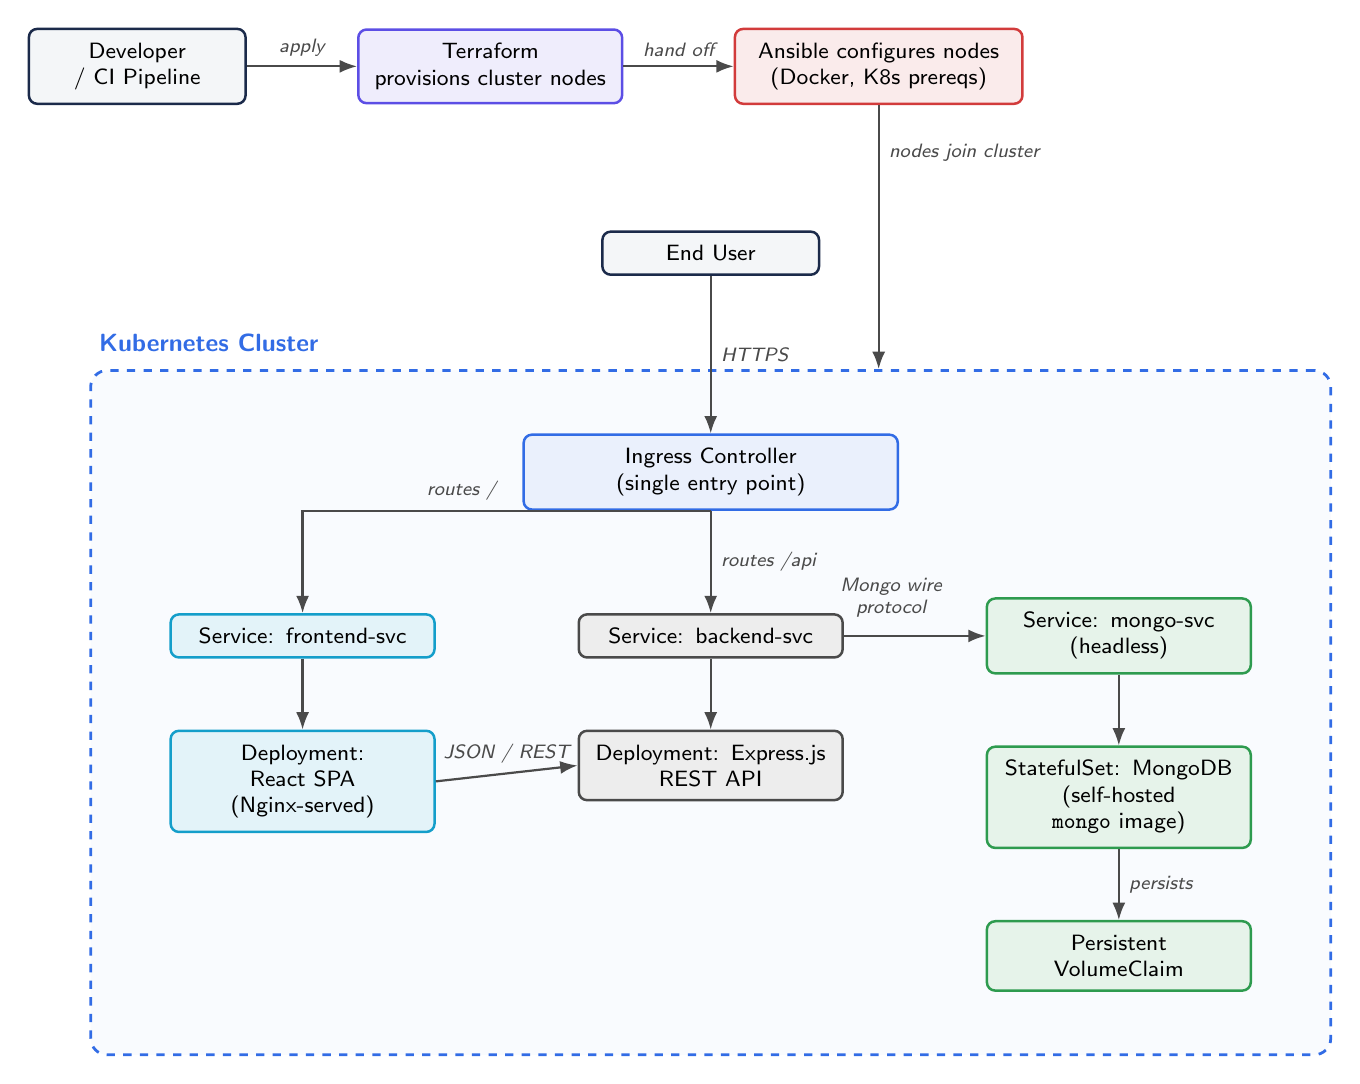
\begin{tikzpicture}[
    font=\sffamily\footnotesize,
    node distance=9mm and 9mm,
    box/.style={rectangle, draw, rounded corners=3pt, align=center, text width=3.0cm, inner sep=5pt, line width=0.9pt},
    infra/.style={box, fill=tfpurple!10, draw=tfpurple},
    cfg/.style={box, fill=ansiblered!10, draw=ansiblered, text width=3.3cm},
    fe/.style={box, fill=reactteal!12, draw=reactteal},
    be/.style={box, fill=expressgray!10, draw=expressgray},
    db/.style={box, fill=mongogreen!12, draw=mongogreen},
    ing/.style={box, fill=k8sblue!10, draw=k8sblue, text width=4.4cm},
    usr/.style={box, fill=lightbg, draw=navy, text width=2.4cm},
    lbl/.style={font=\sffamily\scriptsize\itshape, color=expressgray},
    arr/.style={-{Latex[length=2.2mm]}, line width=0.8pt, color=expressgray},
    cluster/.style={rectangle, draw=k8sblue, dashed, line width=1pt, rounded corners=6pt, fill=k8sblue!3}
]

% --- Kubernetes runtime, built first so the cluster box can fit around it ---
\node[ing] (ingress) {Ingress Controller\\(single entry point)};

\node[be, below=13mm of ingress] (besvc) {Service: backend-svc};
\node[fe, left=18mm of besvc]    (fesvc) {Service: frontend-svc};
\node[db, right=18mm of besvc]   (dbsvc) {Service: mongo-svc\\(headless)};

\node[fe, below=9mm of fesvc] (fepod) {Deployment: React SPA\\(Nginx-served)};
\node[be, below=9mm of besvc] (bepod) {Deployment: Express.js\\REST API};
\node[db, below=9mm of dbsvc] (dbpod) {StatefulSet: MongoDB\\(self-hosted \texttt{mongo} image)};

\node[db, below=9mm of dbpod] (pvc) {Persistent\\VolumeClaim};

% --- Cluster boundary, sized to fit its contents ---
\begin{scope}[on background layer]
\node[cluster, fit=(ingress)(fesvc)(dbsvc)(fepod)(bepod)(pvc), inner xsep=10mm, inner ysep=8mm] (clusterbox) {};
\end{scope}
\node[k8sblue, font=\sffamily\bfseries\small, anchor=south west] at (clusterbox.north west) [yshift=1mm] {Kubernetes Cluster};

% --- Provisioning / config-management chain, above the cluster ---
\node[usr, above=20mm of ingress] (user) {End User};
\node[infra, above=16mm of user, xshift=-28mm] (tf)  {Terraform\\provisions cluster nodes};
\node[usr, left=14mm of tf] (dev) {Developer\\/ CI Pipeline};
\node[cfg, right=14mm of tf] (ans) {Ansible configures nodes\\(Docker, K8s prereqs)};

% --- Arrows: provisioning chain ---
\draw[arr] (dev) -- (tf) node[midway, lbl, above]{apply};
\draw[arr] (tf) -- (ans) node[midway, lbl, above]{hand off};
\draw[arr] (ans.south) -- ++(0,-6mm) -| node[near start, lbl, right]{nodes join cluster} (clusterbox.north -| ans);

% --- Arrows: user request flow ---
\draw[arr] (user) -- (ingress) node[midway, lbl, right]{HTTPS};
\draw[arr] (ingress.south) -| node[near start, lbl, above left]{routes /} (fesvc.north);
\draw[arr] (ingress.south) -- node[midway, lbl, right]{routes /api} (besvc.north);
\draw[arr] (fesvc) -- (fepod);
\draw[arr] (besvc) -- (bepod);
\draw[arr] (fepod.east) -- (bepod.west) node[midway, lbl, above]{JSON / REST};
\draw[arr] (besvc.east) -- (dbsvc.west) node[midway, lbl, align=center, above, xshift=-3mm, yshift=1mm]{Mongo wire\\protocol};
\draw[arr] (dbsvc) -- (dbpod);
\draw[arr] (dbpod) -- (pvc) node[midway, lbl, right]{persists};

\end{tikzpicture}
\end{center}

\vspace{4pt}
\section*{Diagram Notes}
\begin{itemize}
  \item \textbf{Provisioning \& config (top):} Terraform creates the cluster nodes / networking; Ansible then configures each node (container runtime, Kubernetes prerequisites) and joins it to the cluster.
  \item \textbf{Runtime (dashed box):} everything inside the Kubernetes cluster boundary is deployed via manifests — Ingress, three Deployments/StatefulSets, their Services, and one PVC for MongoDB's data directory.
  \item \textbf{Traffic path:} the user only ever talks to the Ingress; it fans requests out to the frontend Service (static routes) and backend Service (\texttt{/api} routes), which in turn talks to MongoDB over the internal cluster network — nothing but Ingress is exposed externally.
\end{itemize}

\vfill
{\small\color{rulegray!60!black}\hrule}
\begin{center}
\small\color{expressgray} Page 2 of 2 --- System Architecture Diagram
\end{center}

\end{document}
